%%%%%%%%%%%%%%%%%%%%%%%%%%%%%%%%%%%%%%%%%%%%%%%%%%%%%%%%%%%%%%%%%%%%%%%%%%%%%%%%
% setup.tex
% Main tex file for setup and content collocation
% For the use of University of Amsterdam
% Information Systems and Data Science students
% Adapted by Riccardo Fiorista (riccardo.fiorista@proton.me)
%%%%%%%%%%%%%%%%%%%%%%%%%%%%%%%%%%%%%%%%%%%%%%%%%%%%%%%%%%%%%%%%%%%%%%%%%%%%%%%%

% Options:
%% `nolinenumbering` - If you want to remove line numbering on submission
%% `draftmargins` - If you would like to give your reviewer more space for comments
\documentclass[]{thesisdesign}

\usepackage[shortlabels]{enumitem}
\setlist[enumerate]{nosep}

%%%%%%%%%%%%%%%%%%%%%%%%%%%%%%%%%%%%%%%%%%%%%%%%%%%%%%%%%%%%%%%%%%%%%%%%%%%%%%%%
% DOCUMENT METADATA
%%%%%%%%%%%%%%%%%%%%%%%%%%%%%%%%%%%%%%%%%%%%%%%%%%%%%%%%%%%%%%%%%%%%%%%%%%%%%%%%

% Thesis related entries
\title{Optimising peregrine for simulation-based inference of gravitational waves}
\subtitle{Submitted on: \textbf{29-02-2024}}

% Author data
\authorname{Nicola Asquith}
\authoremail{nicola.asquith@student.uva.nl}
% ACM-sepecific entries
\affiliation{
    \institution{\thesisinstitution}
    \city{\thesiscity}
    \country{\thesiscountry}
}

% Supervisor data
\authorname{Christoph Weniger}
\authoremail{C.Weniger@uva.nl}
% ACM-sepecific entries
\affiliation{
    \institution{GRAPPA Institute, Institute for Theoretical Physics \\ \thesisinstitution}
    %\city{\thesiscity}
    %\country{\thesiscountry}
}

%%%%%%%%%%%%%%%%%%%%%%%%%%%%%%%%%%%%%%%%%%%%%%%%%%%%%%%%%%%%%%%%%%%%%%%%%%%%%%%%
% tikz library
%%%%%%%%%%%%%%%%%%%%%%%%%%%%%%%%%%%%%%%%%%%%%%%%%%%%%%%%%%%%%%%%%%%%%%%%%%%%%%%%
\usepackage{tikz}
\usetikzlibrary{shapes.geometric, arrows}
\tikzstyle{sample} = [rectangle, rounded corners, minimum width=1cm, minimum height=1cm, text centered, text width=4cm, draw=black, fill=red!30]
\tikzstyle{simulator} = [rectangle, rounded corners, minimum width=1cm, minimum height=1cm, text centered, text width=4cm, draw=black, fill=blue!30]
\tikzstyle{network} = [rectangle, rounded corners, minimum width=1cm, minimum height=1cm, text centered, text width=5cm, draw=black, fill=green!30]
\tikzstyle{inference} = [rectangle, rounded corners, minimum width=1cm, minimum height=1cm, text centered, text width=2cm, draw=black, fill=yellow!40]
\tikzstyle{pinput} = [rectangle, minimum width=1cm, minimum height=1cm, text centered, draw=black, text width=2cm, fill=pink!30]
\tikzstyle{tinput} = [rectangle, minimum width=1cm, minimum height=1cm, text centered, text width=2cm, draw=black, fill=pink!30]
\tikzstyle{output} = [rectangle, minimum width=1cm, minimum height=1cm, text centered, draw=black, fill=orange!30]

\tikzstyle{arrow} = [thick, ->, >=stealth]

%%%%%%%%%%%%%%%%%%%%%%%%%%%%%%%%%%%%%%%%%%%%%%%%%%%%%%%%%%%%%%%%%%%%%%%%%%%%%%%%
% CONTENT
%%%%%%%%%%%%%%%%%%%%%%%%%%%%%%%%%%%%%%%%%%%%%%%%%%%%%%%%%%%%%%%%%%%%%%%%%%%%%%%%
\begin{document}

\pagestyle{plain}
\setcounter{page}{0}
\fixemptypage

\maketitle

% Sections; Try to stick to this setup
\section{Introduction}
\label{sec:introduction}
% Mention scientific context/field, problem statement, research gap and candidate (sub) research question(s). 

Gravitational Waves (GW) are ripples in the fabric of space-time originating from the acceleration of massive astronomical objects e.g. the merger of black holes or neutron stars. Analysis of gravitational wave signals can be used to infer physical information about their source of origin. 

Since the first direct observation of gravitational waves in 2015, there has been a considerable increase in detector sensitivities and survey volumes. The substantial increase in detection rate of events over time is introducing significant data analysis challenges for the gravitational wave community \cite{bhardwaj2023peregrine}.
For instance, current data analysis pipelines are not prepared to deal with independent signals arriving coincidentally in detectors, and scale poorly as the dimensionality of the problem increases \cite{alvey2023things}. This makes the analysis of large number of overlapping signals, or those containing non-stationary noise computationally infeasible.

The \texttt{peregrine} analysis pipeline has been developed at the UvA GRAPPA institute to help address some of these challenges \cite{bhardwaj2023peregrine}. It utilises Simulation-based inference (SBI) based on the TMNRE (Truncated Marginal Neural Ratio Estimation) algorithm and the U-Net convolutional neural network architecture. Due to the high simulation costs associated with running these analysis pipelines, this thesis will focus on the optimisation of the network architecture underlying the \texttt{peregrine} code. The main research question will be: 

\noindent \textit{RQ: To what extent can the optimisation of the \texttt{peregrine} network architecture reduce the simulation budget, while still producing the same results as the original \texttt{peregrine}?}

Smaller sub-questions to be addressed include:

\noindent SRQ1: What parameters have the most influence on the generated/detected gravitational wave signals?

\noindent SRQ2: How can more efficient sampling methods be used to further improve the computational efficiency of \texttt{peregrine}?


\section{Related Work}
\label{sec:related_work}
% Your work needs to be grounded and compared to earlier work and the state-of-the-art. Start the section with announcing the research gap and also end with the research gap. Consider using hypotheses. 
Write about your related work here. Make clear to which key papers you will compare your eventual results. This can be done from the perspective of methods used, the task at hand and the addressed domain.
\section{Methodology}
\label{sec:methodology}
% Focus on what you add to the existing method. Explain what you will do and why (and how). Do not forget to characterize your research design. There should be an evaluation plan in this section. (For DS students, this normally means using manually labelled or ground truth data.)

\subsection{Signal analysis pipeline}

The overall objective of this work is to increase the efficiency of the \texttt{Peregrine} data analysis pipeline. The work will begin with reproducing the results from papers \cite{bhardwaj2023peregrine} and \cite{alvey2023things}, as this will form the benchmark to which the eventual results will be compared to.

The workflow for the simulation-based inference technique for the analysis of the gravitational wave signals as implemented in \texttt{peregrine} \cite{bhardwaj2023peregrine} is shown in Figure \ref{fig:peregrine_pipeline}. The process starts by setting the 15 parameters of the `target observation' and then generating the example waveform to be analysed. This is done so there are `ground-truth' parameter values that you can compare your final posterior probability density distributions with and validate the overall method. If we use a true experimentally measured signal, then we can never know for certain what the `ground-truth' values of the parameters are. Given the accuracy that we can forward model the GW signals with, once the method is validated with the simulated waveforms, it is expected to work equally well with true experimental measurements.

\begin{figure}[htb]
    \centering
    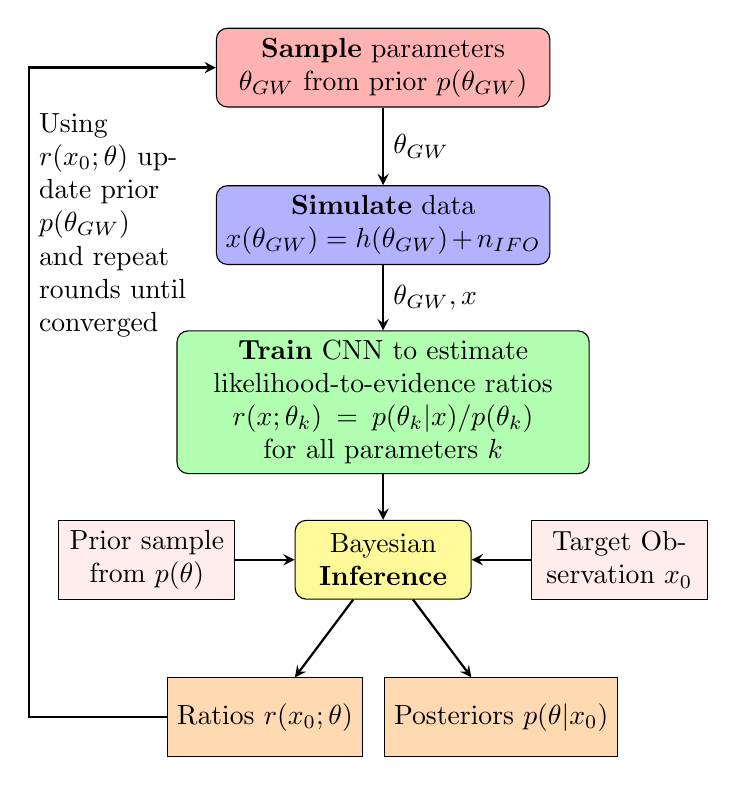
\begin{tikzpicture}[node distance=2cm]
        \node (sampling) [sample] {\textbf{Sample} parameters $\boldsymbol{\theta}_{GW}$ from prior $p(\boldsymbol{\theta}_{GW})$};
        \node (fsimulator) [simulator, below of=sampling] {\textbf{Simulate} data $\boldsymbol{x}(\theta_{GW}) = h(\theta_{GW}) + n_{IFO}$};
        \node (network) [network, below of=fsimulator, yshift=-0.25cm] {\textbf{Train} CNN to estimate likelihood-to-evidence ratios $r(\boldsymbol{x};\theta_k) = p(\theta_k|\boldsymbol{x})/p(\theta_k)$ for all parameters $k$};
        \node (inference) [inference, below of=network] {Bayesian \textbf{Inference}};
        \node (prior) [pinput, left of=inference, xshift=-1cm] {Prior sample from $p(\theta)$};
        \node (target) [tinput, right of=inference, xshift=1cm] {Target Observation $\boldsymbol{x}_0$};
        \node (ratios) [output, below of=inference, xshift=-1.5cm] {Ratios $r(\boldsymbol{x}_0;\theta)$};
        \node (posterior) [output, below of=inference, xshift=1.5cm] {Posteriors $p(\theta|\boldsymbol{x}_0)$};
        \draw [arrow] (sampling) -- node[anchor=west] {$\boldsymbol{\theta}_{GW}$} (fsimulator);
        \draw [arrow] (fsimulator) -- node[anchor=west] {$\boldsymbol{\theta}_{GW},\boldsymbol{x}$} (network);
        \draw [arrow] (network) -- (inference);
        \draw [arrow] (prior) -- (inference);
        \draw [arrow] (target) -- (inference);
        \draw [arrow] (inference) -- (posterior);
        \draw [arrow] (inference) -- (ratios);
        \draw [arrow] (ratios) -- +(-3,0) |- node[anchor=west, yshift=-2cm, text width=2cm]{Using $r(\boldsymbol{x}_0;\theta)$ update prior $p(\boldsymbol{\theta}_{GW})$ and repeat rounds until converged} (sampling);
    \end{tikzpicture}
    \caption{High-level overview of the simulation-based inference method used for this work.}
    \label{fig:peregrine_pipeline}
\end{figure}

\subsection{Data simulation}

The forward simulator to generate the GW waveform data and subsequently used to train the neural network is generated using the Bilby code \cite{Ashton_Bilby_2019} from input parameters that have been randomly sampled from prior distributions. We will investigate whether some more active learning can be introduced to increase the efficiency of the sampling process. For instance, some parameters such as the chirp mass\footnote{The chirp mass is a combination of the two object masses in the binary system, and is a key factor in the gravitational wave frequency as the two objects spiral inwards toward each other.\\$\mathcal{M} = \frac{(m_1 \cdot m_2)^{3/5}}{(m_1 + m_2)^{1/5}}$} may be inferred early on with relatively high confidence, but currently in successive simulation rounds continues to be sampled from a uniform distribution within $\pm5\sigma$ \cite{Miller_TMNRE_2021}. By being more selective in the sampling of parameters that are known with relatively high confidence, we can focus the simulation budget more on the parameters we know with less confidence. To do this in a systematic way, a complete survey of how influential each parameter is on the different segments of the GW signal will be carried-out first.

\subsection{Optimisation of network architecture}

The architecture of the network currently implemented in \texttt{peregrine} is the U-Net architecture \cite{Ronneberger_UNet_2015}. Given the advances in machine learning and CNN architectures since 2015, it is believed that this network can be improved upon. The optimisation of this network architecture will be the main focus of this thesis. 

Investigative studies will be performed to find the best network architectures most suitable for the data format. In this specific case, the data consists of 1D signals in both time and frequency domains, collected from three separate detectors that have captured the event simultaneously. An example of the signal in the time domain is shown in Figure \ref{fig:obs_time_domain}. In total, there are 8192 channels corresponding to 4\,s of collection time at a sampling frequency of 2048\,Hz. Through the Fourier transform, the time signal can be decomposed into its constituent frequency components. Both the time and frequency domains are fed into the network, since they have different information about the GW encoded. An example of the signal in the frequency domain is shown in Figure \ref{fig:obs_freq_domain}.

The chosen network architecture also needs to be capable of segmenting the signal into three components, representing the different stages of the merger event -- inspiral, merger and ringdown \cite{Pan_GW_2014}. Each of the parameters in $\boldsymbol{\theta}_{GW}$ are impacted differently in the different phases \cite{bhardwaj2023peregrine}.

\begin{figure}
  \centering
  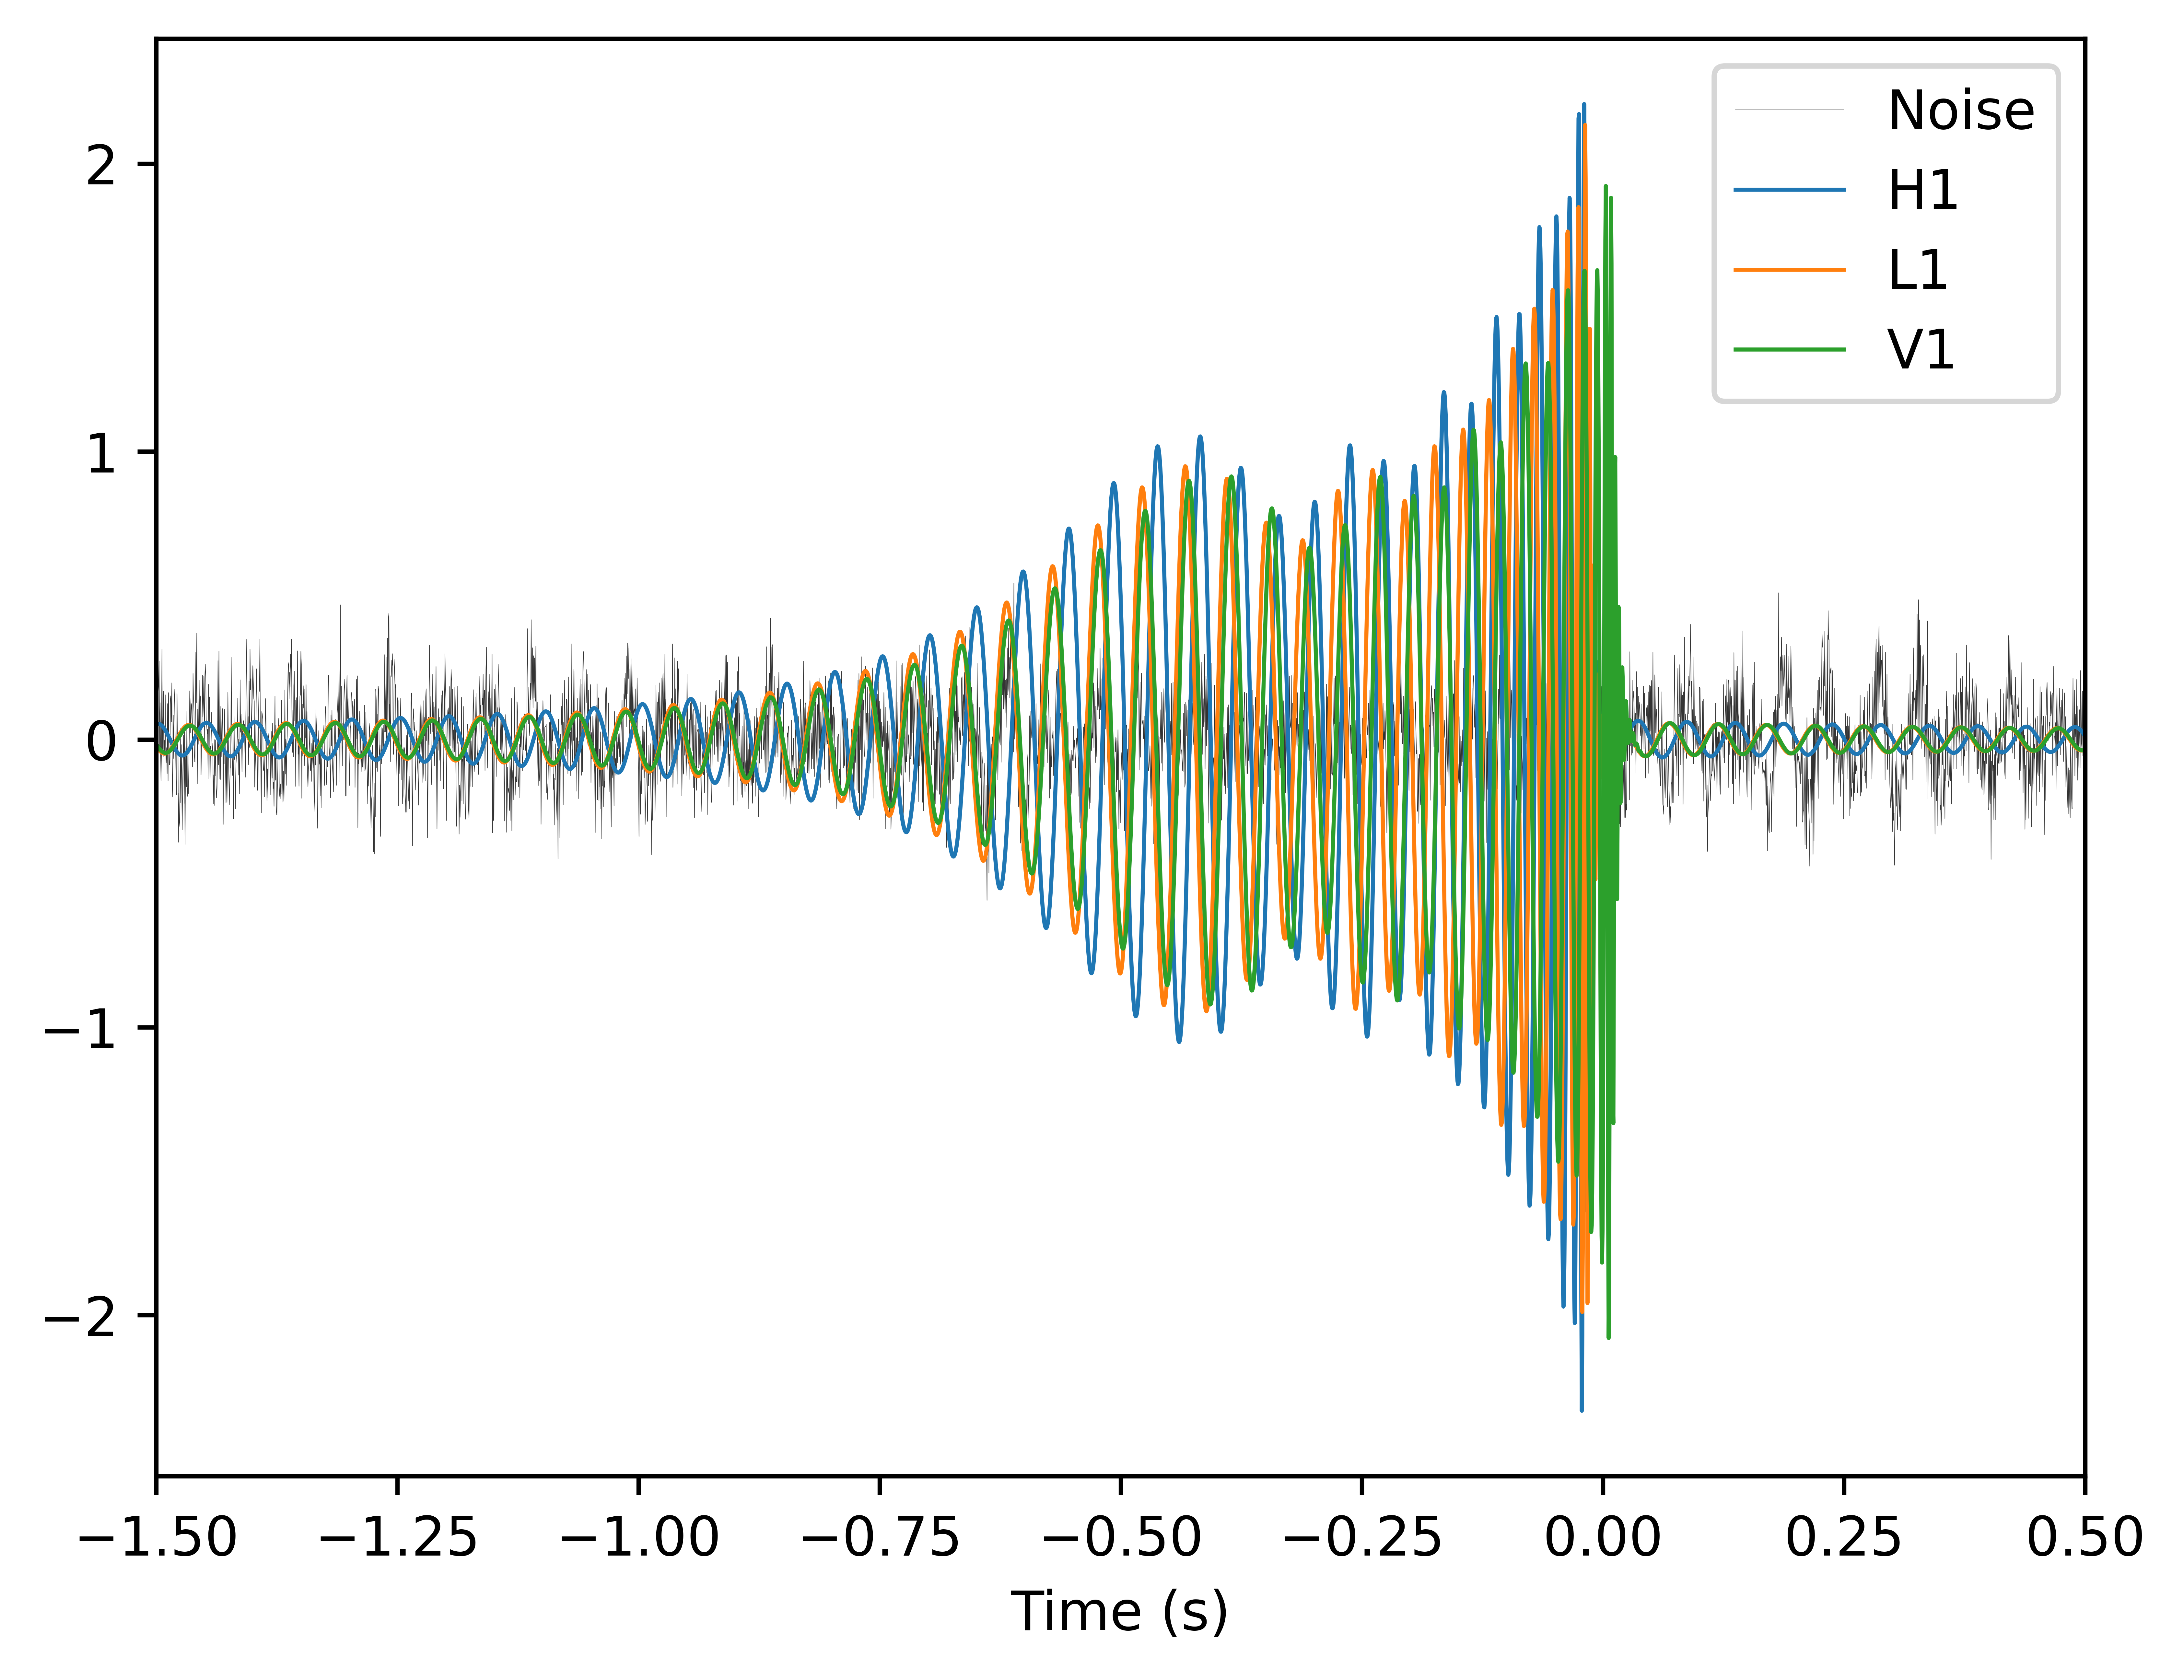
\includegraphics[width=1\linewidth]{media/images/obs_time_domain.png}
  \caption{Example of generated gravitational wave signal in the time domain. Signals from three detectors are shown. For clarity, the noise and signal are shown separately in the figure, but are added together when training the network. The two black holes merge at the moment t=0s. }
  \label{fig:obs_time_domain}
\end{figure}

\begin{figure}
  \centering
  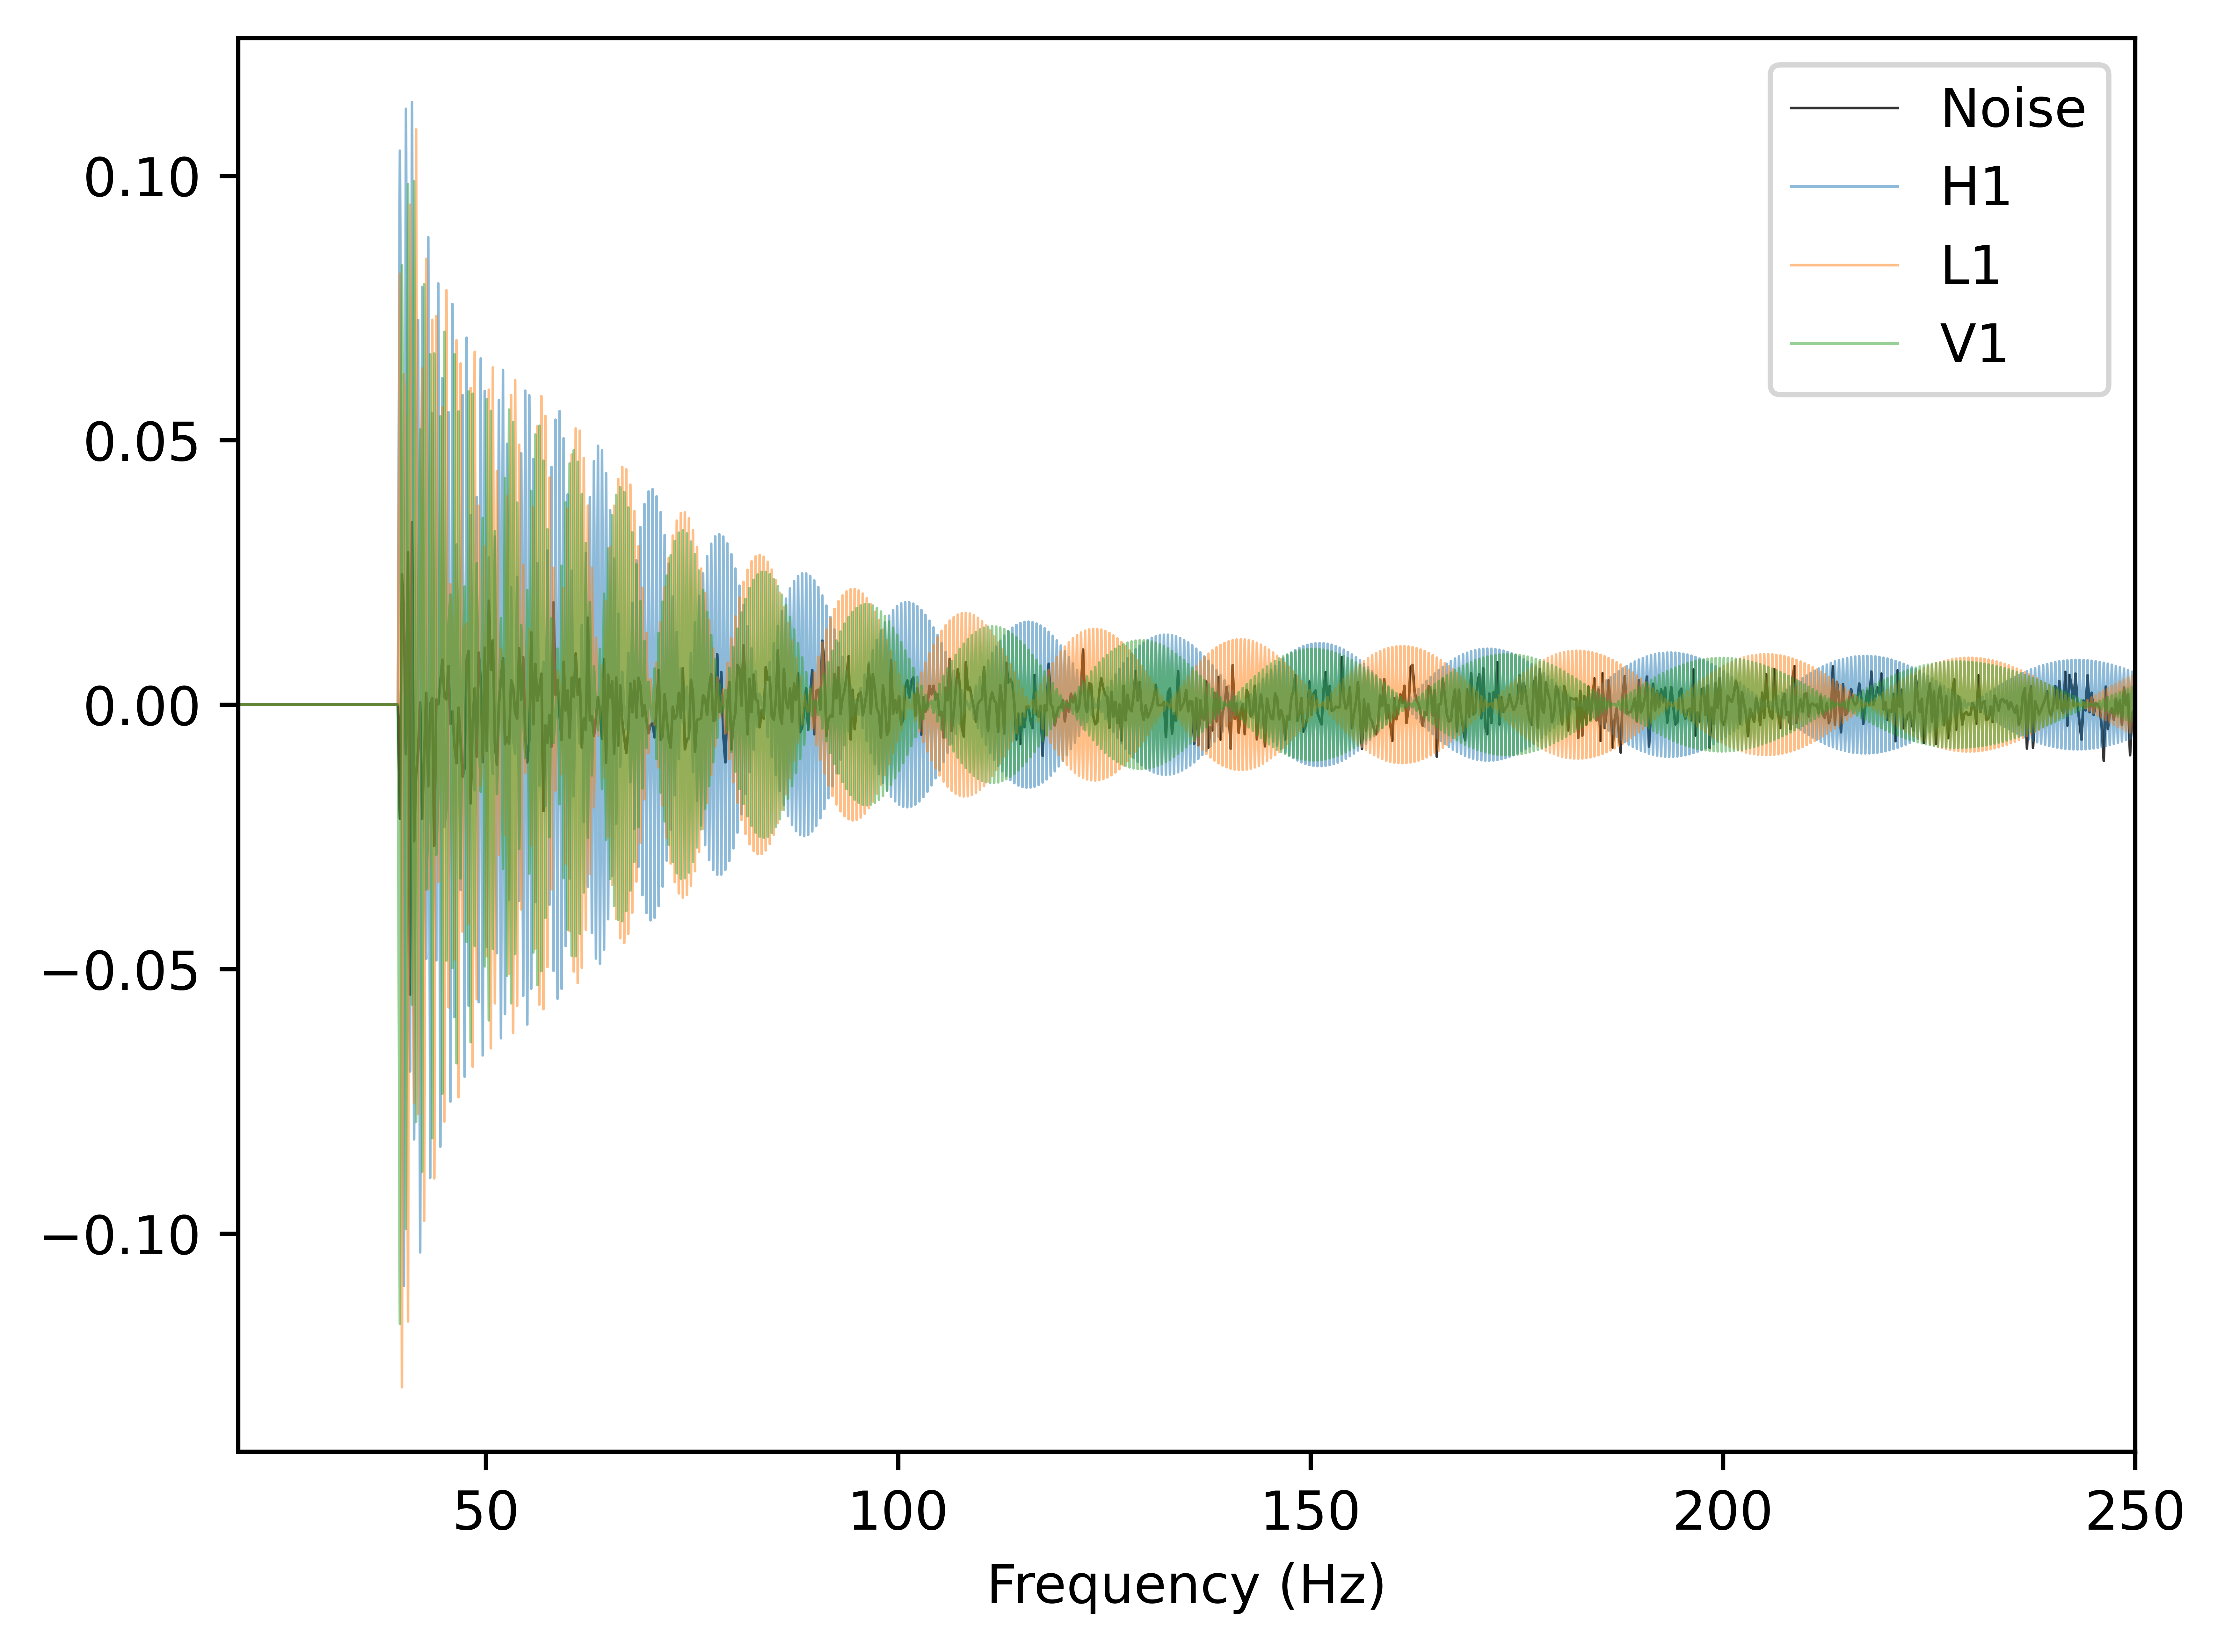
\includegraphics[width=1\linewidth]{media/images/obs_frequency_domain.png}
  \caption{Example of generated gravitational wave signal in the frequency domain. Signals from three detectors are shown. For clarity, the noise and signal are shown separately in the figure, but are added together when training the network.}
  \label{fig:obs_freq_domain}
\end{figure}

\subsection{Evaluation}

The changes to the \texttt{peregrine} analysis pipeline will be fully benchmarked against the original \texttt{peregrine}, both in terms of accuracy of final result and required runtime. The results of the original \texttt{peregrine} have themselves been benchmarked against established likelihood-based methods \cite{Speagle_2020}, and found to be in good agreement. Therefore, in this work we think it is sufficient to compare only with the original \texttt{peregrine}. To demonstrate the applicability of the method to real gravitational wave measurements, if time permits, we will also test the approach using real experimental data.


\section{Risk Assessment}
\label{sec:risk_assessment}
% Describe the risks which you could run into and how you will mitigate them.

The thesis utilises simulated data (not real gravitational wave data) since we are focused on the optimisation of the data analysis pipeline itself, and not the physics of astronomical objects. The `ground-truth' data used for validation of the thesis findings will be the results of papers \cite{bhardwaj2023peregrine} and \cite{alvey2023things}. The risks of using simulated data are mitigated since the data is generated using a method that is well established and accepted by the gravitational wave community for this purpose \cite{alvey2023things}. In addition, if we were to use real experimental data, then we can not know for certain what the true values of the inferred parameters are, making the overall validation less reliable.

Another potential risk is that the required computational effort could exceed the assigned student budget provided for the Snellius cluster. This risk can be mitigated by monitoring the consumed budget throughout the project, or possibly requesting more budget.

\section{Project Plan}
\label{sec:project_plan}
% Describe a timeline via a Gantt chart or table with achievements per week.
Present your timeline here. Finally, you show your academic maturity by being able to quantify how much time your work will take (realistically!). Your UvA supervisor must be able to use your visual timeline to check whether you are on schedule. You can either use a timeline as below or a Gantt chart shown on the right.

% It is important to plan in buffers and time for actually writing the thesis. Do not underestimate the time for the latter, especially as 10 pages do not seem too much (but they are).

% Timeline
% Great and straight forward but lacks documentation. 
% Interested users can have a look here:
% https://github.com/lwiseman/chronology
% Unfortunately, the last commit on main was in 2015
\begin{center}
    \begin{chronology}[1]{0}{13}{60ex}[\linewidth]
        \event[0.01]{1}{Data from Company}
        \event[1]{2}{Feature Engineering}
        \event[2]{3}{Data Enrichment}
        \event[3]{6}{Setup}
        \event[6]{8}{Training}
        \event[8]{9}{Evaluation}
        \event[9]{12}{Writing}
        \event[12]{13}{Buffer}
    \end{chronology}
\end{center}

\newpage

% Gantt Chart
% For more complex Gantt charts see documentation here: 
% http://mirror.ox.ac.uk/sites/ctan.org/graphics/pgf/contrib/pgfgantt/pgfgantt.pdf
\begin{ganttchart}[
    expand chart=0.9\linewidth,
    vgrid,
    hgrid
    ]{0}{12}
        % Titles
        \gantttitle{Weeks}{13} \\
        \gantttitlelist{1,...,13}{1} \\

        % Group
        \ganttgroup{Data Aggregation}{0}{2} \\  % elem 0
        % Concrete tasks
        \ganttbar{Data from Company}{0}{0} \\  % elem 1
        \ganttbar{Feature Engineering}{1}{1} \\  % elem 2
        \ganttbar{Data Enrichment}{2}{2} \\  % elem 3
        % More groups, further tasks ommitted
        \ganttgroup{Setup}{3}{5} \\  % elem 4
        \ganttgroup{Training}{6}{7} \\  % elem 5
        \ganttgroup{Evaluation}{8}{8} \\  % elem 6
        \ganttmilestone{Finish Experiments}{8} \ganttnewline % elem 7
        \ganttgroup{Writing}{9}{11} \\  % elem 8
        \ganttgroup{Buffer}{12}{12} % elem 9
        
        % Connectors
        \ganttlink{elem0}{elem4}
        \ganttlink{elem4}{elem5}
        \ganttlink{elem5}{elem6}
        \ganttlink{elem6}{elem7}
        \ganttlink{elem7}{elem8}
  \label{ganttchart}
\end{ganttchart}


\bibliographystyle{ACM-Reference-Format}
\bibliography{bibliographies/references}

\end{document}

%%%%%%%%%%%%%%%%%%%%%%%%%%%%%%%%%%%%%%%%%%%%%%%%%%%%%%%%%%%%%%%%%%%%%%%%%%%%%%%%
%%%%%%%%%%%%%%%%%%%%%%%%%%%%%%%%%%%%%%%%%%%%%%%%%%%%%%%%%%%%%%%%%%%%%%%%%%%%%%%%